\chapter{\ifenglish Conclusions and Discussions\else บทสรุปและข้อเสนอแนะ\fi}

\section{\ifenglish Conclusions\else สรุปผล\fi}

โครงงาน Flowy: Rent hourly for reading \& co-working จัดทำขึ้นเพื่อแก้ไขปัญหาพื้นที่หรือที่นั่งไม่เพียงพอในการทำกิจกรรมต่าง ๆ ตามความต้องการของผู้ใช้งาน โดยโครงงานนี้สามารถแบ่งการสรุปออกมาได้ 2 หมวดหมู่ได้แก่ ด้านเทคนิคและด้านธุรกิจ

\subsubsection{ด้านเทคนิค}
ผลสรุปของด้านเทคนิคนั้นถือว่าทีมผู้พัฒนานั้นสามารถทำออกมาได้สมบูรณ์แบบตามความต้องการ ทั้งในเรื่อง UI/UX ก็ดีหรือ functionality ของตัวแอปพลิเคชันทั้ง 2 ก็ดี แน่นอนว่ามีรายละเอียดบางจุดที่สามารถพัฒนาให้ดีขึ้นหรือแก้ไขเพิ่มเข้าไปภายหลังได้ แต่เนื่องด้วยข้อจำกัดของเวลาทางผู้พัฒนาจึงตั้งสินใจทำ feature ที่สำคัญเท่าที่จำเป็นก่อน แม้ว่าทีมผู้พัฒนาจะมีแนวความคิดการพัฒนาผลิตภัณฑ์ออกมาในรูปแบบของ Minimum Viable Product (MVP) อยู่แล้ว แต่ผลลัพธ์ที่ตั้งใจทำออกมาก็เกินจุดที่จะเรียกว่า MVP ไปอยู่พอสมควร

\subsubsection{ด้านธุรกิจ}
ผลสรุปของด้านธุรกิจนั้นถือว่าบรรลุเป้าหมายเพียง 70\% เท่านั้น โดย 30\% ที่เหลือที่ไม่สามารถบรรลุได้นั้นคือการให้โฮสต์ (Flowider) เข้ามาใช้บริการในฐานะ contributor ให้ได้มากที่สุดเพื่อที่จะได้ทำการ public launch ต่อไปตามแผนที่วางไว้ในตอนต้น แต่เนื่องด้วยระยะเวลาของการพัฒนาที่พยายามจะส่งมอบ feature ต่าง ๆ ที่จำเป็นให้ฝั่ง Flowider ให้ได้มากที่สุด จึงทำให้กินระยะเวลาของการทดสอบดังกล่าวไปโดยสรุปทั้งหมด ณ ปัจจุบันที่รายงานฉบับนี้ได้เขียนอยู่ แอปพลิเคชันทั้ง 2 นั้นสามารถใช้การทุก feature ที่จำเป็นและเป็นพื้นฐานได้อย่างครบถ้วนและสามารถที่จะแก้ไขหรือพัฒนาต่อไป โดยในอนาคตทางผู้พัฒนามีความตั้งใจที่จะพัฒนาต่อและทำให้ Flowy นี้สามารถเป็นธุรกิจที่เข้ามาตอบโจทย์ความต้องการของผู้ที่มองหาพื้นที่ในการทำงาน, อ่านหนังสือ หรือทำกิจกรรมอื่น ๆ ต่อไปตามแผนที่วางไว้ในตอนต้น

\section{\ifenglish Challenges\else ปัญหาที่พบและแนวทางการแก้ไข\fi}

\subsubsection{Flowider มีน้อย เนื่องด้วยเหตุผลทางธุรกิจ}
เนื่องด้วย Flowy เป็นแอปพลิเคชันแพลตฟอร์ม จึงหมายความว่าเราต้องทำงานกับ stakeholder มากกว่า 1 ฝ่าย ซึ่งในที่นี่ Flowy ต้องทำงานกับ 2 ฝ่ายหลักด้วยกันคือฝั่งของ Flowy (ผู้เช่า) และ Flowider (โฮสต์) โดยในส่วนของ Flowider นั้นเป็นข้อจำกัดของโครงงานนี้ เนื่องจากทีมผู้พัฒนาได้ทำการติดต่อผ่านการโทรศัพท์ไปติดต่อเจรจากับเจ้าของพื้นที่นั้น ๆ เพื่อเชิญชวนให้เขาเข้ามาเป็นส่วนหนึ่งกับเรา

แต่ผลการเจรจานั้นส่วนใหญ่แล้วจะไม่ประสบความสำเร็จเนื่องจากปัญหาเรื่องความเชื่อใจและความปลอดภัยของข้อมูลส่วนบุคคลที่จะเข้ามาสู่แพลตฟอร์มของเรา หรือในความเห็นผู้พัฒนาเองก็คิดว่าเนื่องด้วยเรายังมีสถานะเป็นนักศึกษาอยู่จึงทำให้ความเชื่อมั่นหรือความมั่นใจที่จะเข้าร่วมนั้นมีไม่พอที่จะทำให้ Flowider ตัดสินใจเข้าร่วม

โดยแนวทางวิธีการแก้ไขปัญหานี้คือ เราจำเป็นต้องหาผู้ที่มีเงื่อนไขในการเข้าร่วมน้อยกว่านี้ ซึ่งอาจเปลี่ยนจากการเชิญชวนกลุ่มสถานที่ที่มีอุปสงค์เยอะอยู่แล้ว เช่น ร้านกาแฟ, โคเวิร์กกิ้งสเปซ ฯลฯ เป็น กลุ่มสถานที่ส่วนบุคคล เช่น บ้านหรือคอนโดมิเนียมแทน เพื่อให้การปล่อยเช่าของเขาสร้างรายได้นั้นลดกำแพงเงื่อนไขลง จนเมื่อเรามี Flowider ประเภทนี้มากเพียงพอแล้ว เราจึงจะมีเสียงในการต่อรองหรือเชิญชวนกลุ่มสถานที่อื่นอย่างร้านกาแฟ, โคเวิร์กกิ้งสเปซ เข้ามาบนแพลตฟอร์มของ Flowy

และอีกแนวทางหนึ่งคือควรเผื่อเวลาไว้สำหรับการเข้าไปเจรจาตัวต่อตัวด้วย ซึ่งทางทีมผู้พัฒนาไม่ได้เผื่อเวลาในส่วนนี้เพียงพอ

\subsubsection{ระบบ Search \& Filter}
เดิมแล้ว Flowy ตั้งใจที่จะทำระบบ Search \& Filter อย่างที่แพลตฟอร์มอื่น ๆ ที่มีลักษณะใกล้เคียงกันมี ซึ่งเมื่อเราทำออกมาแล้วแต่ยังมีจำนวนของ Flowider บนแพลตฟอร์มไม่เพียงพอ เราพบว่าทำให้ประสบการณ์การใช้งานนั้นไม่ค่อยดีเพราะเมื่อทำการค้นหาแล้วบางครั้งก็ไม่พบสถานที่ที่ตรงกับความต้องการ เราจึงแก้ไขปัญหานี้เฉพาะหน้าด้วยการเพิ่มส่วนทักทายผู้ใช้งานไปก่อน จนเมื่อเรามี Flowider มากเพียงพอแล้วจึงจะเปิดใช้ feature นี้อีกครั้งหนึ่ง
\begin{figure}[h]
    \begin{center}
    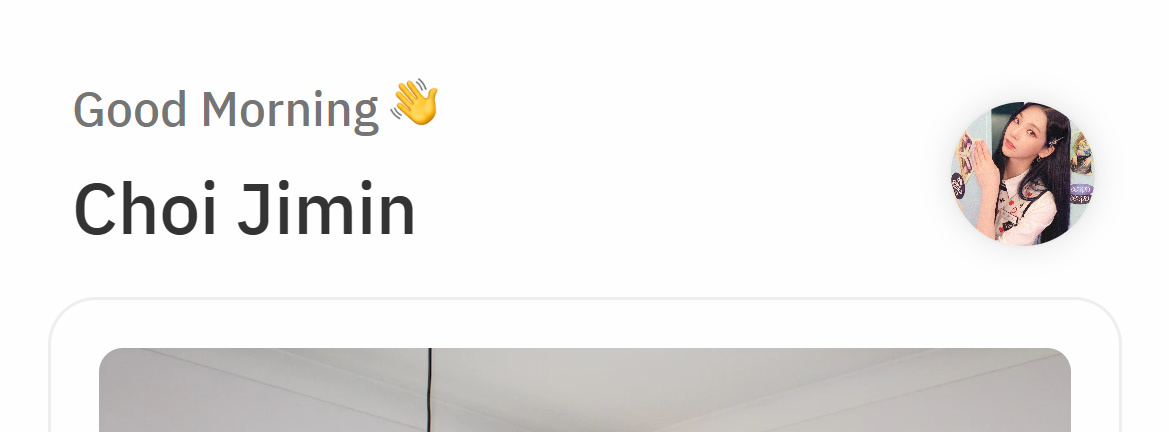
\includegraphics[width=4in]{./image/welcome_bar.png}
    \end{center}
    \caption[Welcome bar]{รูปภาพส่วนทักทายผู้ใช้งานดังกล่าว}
    \label{fig:welcome_bar}
\end{figure}

\section{\ifenglish%
Suggestions and further improvements
\else%
ข้อเสนอแนะและแนวทางการพัฒนาต่อ
\fi
}
ในส่วนของ Flowy และ Flowider ควรที่จะพัฒนา UI/UX ให้ดีขึ้นกว่านี้เพื่อการใช้งานที่มีประสิทธิภาพ หน้าตา interface ที่สวยงาม และมอบประสบการณ์การใช้งานที่ดีให้กับ user โดยอาศัยการเข้าไปทดสอบและพูดคุยถึงปัญหาและความต้องการของ user ให้สม่ำเสมอและนำหลักการออกแบบมาใช้

ซึ่งจากประเด็นดังกล่าว เรานำมาต่อยอดในเรื่องของการให้บริการของเราที่ปัจจุบันนั้นมีบริษัทหลายแห่งที่มีระบบ Point-of-Sell (POS) เช่น Grab, Lineman ฯลฯ ซึ่งหากเราจะเป็นหนึ่งในบริษัทเหล่านั้นที่ต้องการให้ Flowider ใช้งาน POS ของเราอีกหนึ่งเครื่อง อาจเป็นตัวเลือกที่ไม่ค่อยดีนักเพราะผู้ใช้งานต้องทำงานกับอุปการณ์มากชิ้น โดยอาจารย์พฤษภ์ บุญมาได้ให้คำแนะนำว่าเราควรที่จะไป integrate หรือเชื่อมต่อระบบกับผู้ให้บริการเหล่านั้นดังที่กล่าวสักหนึ่งเจ้า ให้เป็นความร่วมมือทางธุรกิจที่สามารถสร้างประโยชน์ได้ทุกฝ่าย ซึ่งเราก็ไม่จำเป็นต้องให้ Flowider ใช้ระบบ POS ของเราอีกแล้ว ลดต้นทุนการผลิตลง, พันธมิตรธุรกิจของเราก็ได้เพิ่มโอกาสทางธุรกิจใน sector อื่น ๆ และสุดท้ายผู้ใช้งานก็มีประสบการณ์ใช้งานที่ดี ไม่จำเป็นต้องทำงานกับอุปกรณ์หลายชิ้นอีกต่อไป
